% !Mode:: "TeX:UTF-8"
% !TEX root = ..\Literature_Translation.tex
\stepcounter{app}
\setcounter{figure}{0}
\setcounter{table}{0}
\newpage
\begin{Abstract}
\chapter*{航空工厂的装配夹具生产调度}\addcontentsline{toc}{section}{航空工厂的装配夹具生产调度}
\begin{center}
\vspace{2mm}
{
 {\xiaosi Bruno Jensen Virginio da Silva$^a$,  Reinaldo Morabito$^a$, Denise Sato Yamashita$^a$,\\ Horacio Hideki Yanasse$^b$}

 {\xiaowu $^a$Departamento de Engenharia de Produção, Universidade Federal de São Carlos, Brazil\\
 $^b$Nati Instituto de Ciência e Tecnologia, Universidade Federal de São Paulo, Brazil}
}
\end{center}
{\songti
\noindent \xiaowu\textbf{摘要:}本文探讨了在某机械工厂装配车间内的生产调度问题。该装配工艺包含两个工段:在工段1,所需零件在一批同速机上同时装配,并且这些同速机的准备时间也相同;装配完成的部件进入工段2 进,并在不同的异速机上进行系统集成组装。同速机和异速机在切换生产产品簇的时候都需要考虑换线时间。本文建立了一个混合整数规划(MIP) 模型以求解小型问题,并提出了用于求解中、大型问题的三个启发式方法。经过计算检验,相比较其余两个方法,其中一个利用滚动时域调度策略的整批产品簇排序启发式组合的方法(RFBFS),在解决问题方面有较高质量。实践表明,RFBFS方法确实显著优于现行方法。

\keywords{混合整数规划、作业划分、批量作业、产品簇调度}
}
\end{Abstract}
\kchapter{haha}
计算检验,相比较其余两个方法,其中一个利用滚动时域调度策略的整批产品簇排序启发式组合的方法(RFBFS),在解决问题方面有较高计算检验,相比较其余两个方法,其中一个利用滚动时域调度策略的整批产品簇排序启发式组合的方法(RFBFS),在解决问题方面有较高计算检验,相比较其余两个方法,其中一个利用滚动时域调度策略的整批产品簇排序启发式组合的方法(RFBFS),在解决问题方面有较高
\begin{gather}
\text{Minimize}\qquad \alpha C_{\max}+\beta\sum_{j=1}^n C_{2,[j]}+\gamma\sum_{j=1}^n T_j \label{equ:8}
\end{gather}
计算检验,相比较其余两个方法,其中一个利用滚动时域调度策略的整批产品簇排序启发式组合的方法(RFBFS),在解决问题方面有较高计算检验,相比较其余两个方法,其中一个利用滚动时域调度策略的整批产品簇排序启发式组合的方法(RFBFS),在解决问题方面有较高计算检验,相比较其余两个方法,其中一个利用滚动时域调度策略的整批产品簇排序启发式组合的方法(RFBFS),在解决问题方面有较高
\begin{table}[h]
  \centering\xiaowu
  \caption{MIP 和3个启发式方法的ARPD 比较}
    \begin{tabular}{ccccccccc}
    \toprule
    \multirow{2}[4]{*}{示例编号} & \multicolumn{2}{c}{MIP} & \multicolumn{2}{c}{EDD} & \multicolumn{2}{c}{FBEDD} & \multicolumn{2}{c}{FBFS} \\
   \cline{2-9}
          & Z     & time(s) & Z     & ARPD  & Z     & ARPD  & Z     & ARPD \\
      \midrule
    1     & 331.04 & 10    & 423.64 & 27.97 & 375.92 & 13.56 & 331.04 & 0 \\
    2     & 374.56 & 15    & 435.88 & 16.37 & 396.88 & 5.96  & 376.48 & 0.51 \\
    3     & 338.72 & 21    & 425.64 & 25.66 & 380.08 & 12.21 & 344.48 & 1.7 \\
    4     & 332.4 & 123   & 399.48 & 20.18 & 354.32 & 6.59  & 338.16 & 1.73 \\
    5     & 377.28 & 35    & 435.84 & 15.52 & 395.2 & 4.75  & 377.28 & 0 \\
    6     & 342.64 & 47    & 441.2 & 28.76 & 393.68 & 14.9  & 342.64 & 0 \\
    7     & 316.64 & 24    & 414.64 & 30.95 & 349.64 & 10.42 & 316.64 & 0 \\
    8     & 345.36 & 22    & 443.28 & 28.35 & 391.48 & 13.35 & 345.36 & 0 \\
    9     & 359.04 & 35    & 451.04 & 25.62 & 399.44 & 11.25 & 359.04 & 0 \\
    10    & 386.72 & 8     & 442.56 & 14.44 & 432.8 & 11.92 & 389.04 & 0.6 \\[3pt]
    平均值   & 350.44 & 34    & 431.32 & 23.38 & 386.94 & 10.49 & 352.02 & 0.45 \\
    \bottomrule
    \end{tabular}
\end{table}

计算检验,相比较其余两个方法,其中一个利用滚动时域调度策略的整批产品簇排序启发式组合的方法(RFBFS),在解决问题方面有较高计算检验,相比较其余两个方法,其中一个利用滚动时域调度策略的整批产品簇排序启发式组合的方法(RFBFS),在解决问题方面有较高计算检验,相比较其余两个方法,其中一个利用滚动时域调度策略的整批产品簇排序启发式组合的方法(RFBFS),在解决问题方面有较高
\begin{figure}[h]
\begin{floatrow}[2]
\centering
\ffigbox{\caption{当前制造流程}}{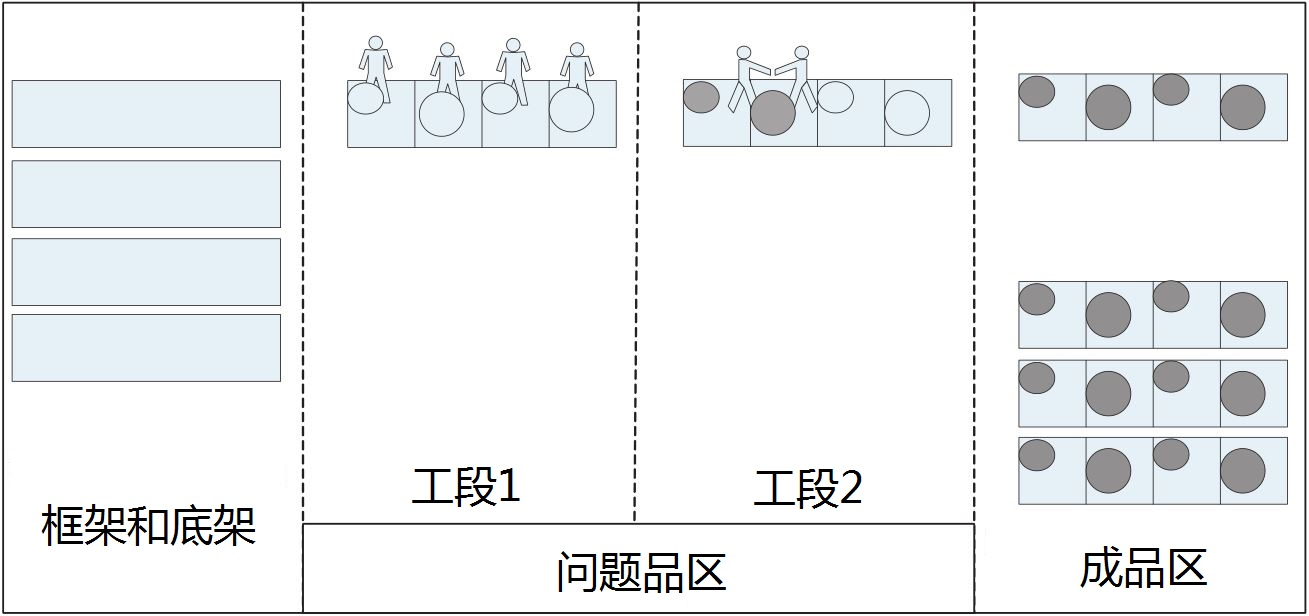
\includegraphics[width=8cm]{current_work_flow.jpg}}
\ffigbox{\caption{运用了作业划分和批量作业的制造流程}}{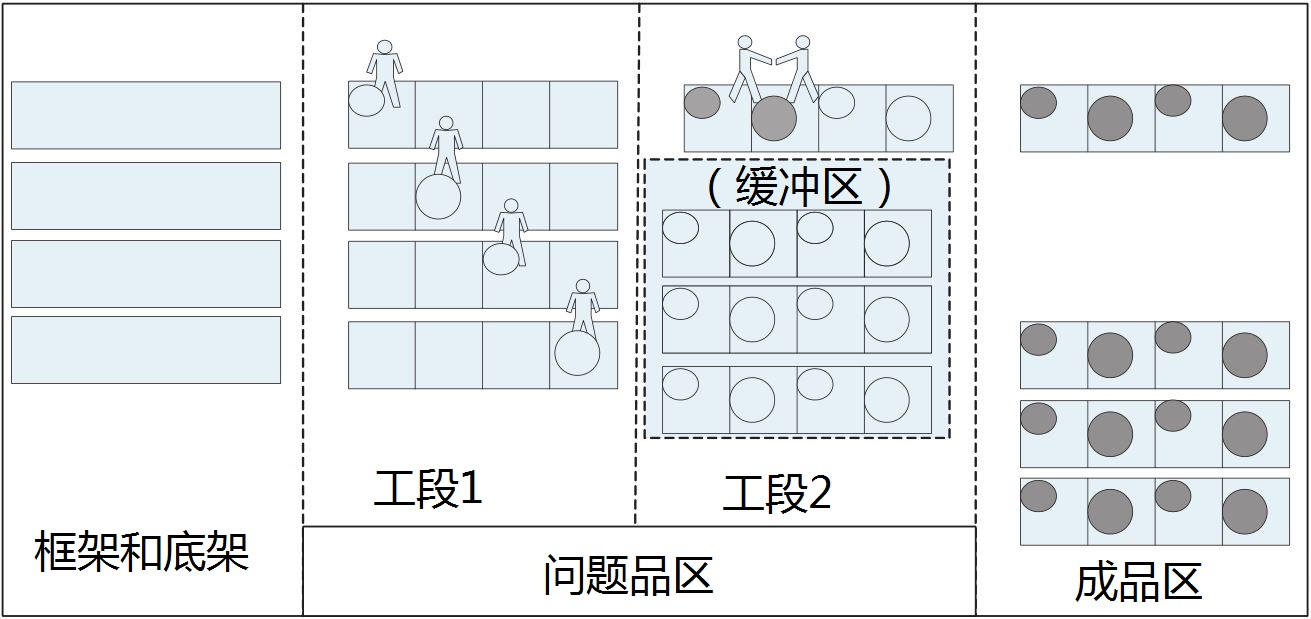
\includegraphics[width=8cm]{batch_work_flow.jpg}}
\end{floatrow}
\end{figure}